\documentclass{standalone}
\usepackage{tikz}
\usetikzlibrary{backgrounds}
\begin{document}
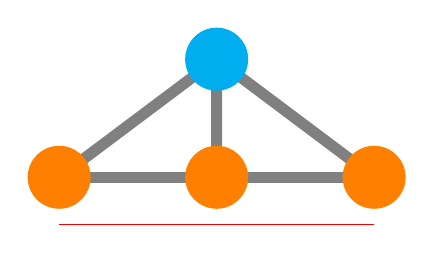
\begin{tikzpicture}
  \foreach \i/\x in {1/0, 2/2, 3/4}
    \fill[orange] (\x,0) circle [radius=0.4] coordinate (c\i);
  \fill[cyan] (2,1.5) circle [radius=0.4] coordinate (top);
  % Drawn after the circles, painted behind them.
  \begin{pgfonlayer}{background}
    \draw[line width=4pt, gray] (c1) -- (top) -- (c3) (c2) -- (top);
    \draw[line width=4pt, black!50] (c1) -- (c3);
  \end{pgfonlayer}
  \draw[red] (0,-0.6) -- (4,-0.6);
\end{tikzpicture}
\end{document}
